\documentclass[12pt]{article}


\usepackage[dvips,letterpaper,margin=0.75in,bottom=0.5in]{geometry}
\usepackage{cite}
\usepackage{slashed}
\usepackage{graphicx}
\usepackage{amsmath}

\begin{document}

\title{DC and Transient Responses of Capacitors and Inductors}

\maketitle

\section{Pre-lab Calculations}

1) For a voltage divider with both resistors of equal value ($R_1=R_2$), what is the ratio of the output voltage to the input voltage ($V_{~\rm out} / V_{~\rm in}$)? \\ \vskip 0.2cm
\noindent
2) Calculate the $RC$ time constant for the circuit in Fig.~\ref{fig:squarerc}.\\ \vskip 0.2cm
\noindent
3) Calculate the $L/R$ time constant for the circuit in  Fig.~\ref{fig:squarelr}.\\

\section{Introduction}

In this lab, you will become familiar with more essential electronics lab equipment:  function generators and oscilloscopes, as well as additional features of your digital multimeter (DMM).  You will experimentally verify the DC and transient response of $RC$ and $RL$ circuits.

\section{Oscilloscope and Function Generator}

In this lab, you will start using your oscilloscope and function generator.  The function generator can be configured to produce any arbitrary function, but the most commonly used are alternating current (sine wave), saw tooth function, and square wave.  Meanwhile, your oscilloscope is used to measure the voltage as a function of time of any signal.

A common mistake made by new experimenters is try to to do too much before obtaining any feedback from their apparatus.  The main problem with this approach is that when something isn't working, it's not clear what component, or what step in the chain, has failed.  Experienced researchers obtain feedback from their apparatus whenever possible.  And the scope is a great way to obtain feedback.  It is a good habit to begin every electronic lab session by looking first at the output of your function generator directly with your oscilloscope.  This ensures that both are working as you expect, and, perhaps more importantly, puts you in the right mindset to look at your circuit at each step along the way.

Make certain that the load impedance setting for your function generator is set to $50~\rm{\Omega}$ and generate a $1~\rm kHz$, $4~\rm V$ peak-to-peak sine wave.  Using the function generator as the AC voltage source, build the simple circuit in Fig.~\ref{fig:acscope} for $R=50~\rm{\Omega}$.  This is the load that the function generator is expecting, based on your setting, so you should get a $4 V$ peak-to-peak voltage across the resistor. 

Confirm this with your oscilloscope.  The oscilloscope is designed to measure the absolute potential relative to ground.  {\bf The only valid place to connect the ground shield from the scope probe is to the ground in your circuit.}  Connect the ground shield of the scope probe to $P_1$ and the probe to $P_2$, then configure your oscilloscope to observe the $4 V$ peak-to-peak signal.

Explore the measurements menu of your scope and configure to measure both the peak-to-peak and root-
mean-square (RMS) of the signal.  What is the RMS of this $4 V$ peak-to-peak signal?

Your DMM is also capable of measuring an AC voltage.  Place your DMM in AC voltage measurement mode and measure the voltage across points $P_1$ and $P_2$.  Are these two instruments in agreement?

Now replace the resistor in your circuit with an $82~\rm{k\Omega}$ resistor and repeat the measurements of the AC voltage across the resistor.  By what factor has the voltage changed?

Change the setting of your function generator to high impedance output, and set the AC voltage back to $4 V$.  Now what do you observe with the scope and DMM?  

Using your knowledge of voltage dividers, see if you can describe what just happened!

\begin{figure}[htbp]
\begin{center}
\begin{picture}(100,100)
\put(0,0){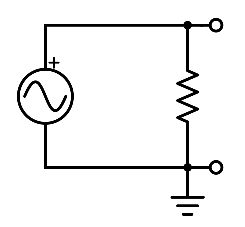
\includegraphics[height=0.15\textheight]{figs/acscope.pdf}} 
\put(5,35){$\widetilde{V}$}
\put(70,55){$R$}
\put(100,35){$P_{1}$}
\put(100,80){$P_{2}$}
\end{picture}
\end{center}
\caption{\label{fig:acscope} Circuit diagram with resistors in series and parallel.}
\end{figure}

\section{DC response of capacitors}

Obtain a resistor with value $R=1.5~\rm k\Omega$ and measure its resistance using your DMM.

Put the function generator to the side for now and use your DC voltage sources for this section.
Build the circuit in Fig.~\ref{fig:dividers}a using the resistor you already obtained, $V=1 ~\rm V$, and a capacitor with $C=.01~\rm\mu F$.

Measure the voltage across the resistor $R$ with your DMM.  Measure it with the scope as well.  What current is flowing through this resistor?  Does the name ``DC blocking capacitor" make sense in this context?

Now build the circuit in Fig.~\ref{fig:dividers}b using $R_1=R_2=R$ and the same components from part a.  What is the voltage across the resistor $R_2$?  What current is passing through the resistor $R_2$?   
Has the parallel capacitor had any effect on the DC voltage divider?

What is the equivalent resistance of a capacitor in a DC circuit?

\begin{figure}[htbp]
\begin{center}
\begin{tabular}{c@{\hskip 1in}c}%\mu F}
\begin{picture}(110,130)
\put(0,0){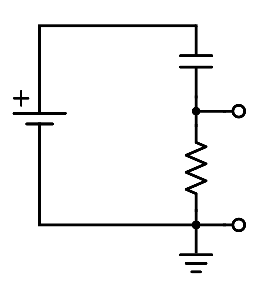
\includegraphics[height=0.20\textheight]{figs/dcrcser.pdf}} 
\put(-8,70){$V$}
\put(75,55){$R$}
\put(75,105){$C$}
\put(114,38){$P_{1}$}
\put(114,70){$P_{2}$}
\end{picture}
&
\begin{picture}(140,130)
\put(0,0){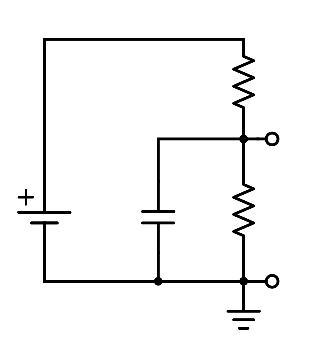
\includegraphics[height=0.20\textheight]{figs/dcrcpar.pdf}}
\put(-5,65){$V$}
\put(45,55){$C$}
\put(78,55){$R_2$}
\put(78,105){$R_1$}
\put(115,38){$P_{1}$}
\put(115,80){$P_{2}$}
\end{picture}\\
(a) & (b) \\
\end{tabular}
\end{center}
\caption{\label{fig:dividers} Circuit diagrams for (a) a DC-blocking capacitor (b) a bypass capacitor.}
\end{figure}

\section{\label{sec:rc} Transient Response of Capacitors}

The square wave mode of your function generator is equivalent to turning on and off a DC voltage.  This allows us to examine the transient response of a circuit. Set the function generator to produce a square wave with frequency $10~\rm kHz$ and voltage with a \textit{high level} of $1~\rm V$ and a \textit{low level} of $0~\rm V$.

Build the circuit shown in Fig.~\ref{fig:squarerc}, using the same values as in the previous section. With the scope ground shield {\em always} plugged into ground at $P_1$ verify that the output of the function generator is indeed a square wave.

Now measure the voltage as a function of time at the point $P_2$.  

Measure the RC time constant and compare to your pre-lab calculation. Be sure to measure the capacitance and the resistance of your components to see if they match.

\begin{figure}[htbp]
\begin{center}
\begin{picture}(110,160)
\put(0,0){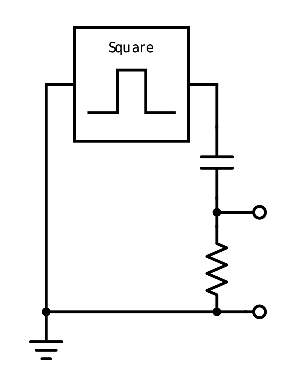
\includegraphics[height=0.25\textheight]{figs/squarerc.pdf}} 
\put(80,90){$C$}
\put(80,55){$R$}
\put(115,65){$P_2$}
\put(115,20){$P_1$}
\end{picture}
\end{center}
\caption{\label{fig:squarerc} Circuit diagram with resistors in series and parallel.}
\end{figure}


\section{\label{sec:rl} Transient Response of Inductors}

Build the circuit shown in Fig.~\ref{fig:squarelr}, with $L=150~\rm\mu H$ and $R=100~\rm\Omega$, and adjust the frequency of the function generator to $100~\rm kHz$, keeping the output voltage levels the same. With the scope ground shield {\em always} plugged into ground at $P_1$ verify that the output of the function generator is indeed a square wave.

Measure the transient response time constant and compare it to your prelab calculation.

\begin{figure}[htbp]
\begin{center}
\begin{picture}(110,160)
\put(0,0){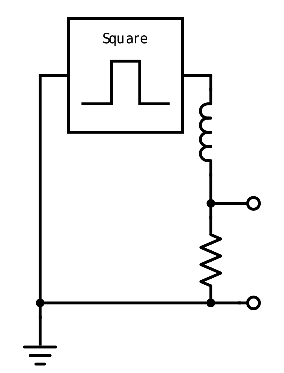
\includegraphics[height=0.25\textheight]{figs/squarelr.pdf}} 
\put(80,90){$L$}
\put(80,55){$R$}
\put(115,65){$P_2$}
\put(115,20){$P_1$}
\end{picture}
\end{center}
\caption{\label{fig:squarelr} Circuit diagram with resistors in series and parallel.}
\end{figure}

\section{Lab Report}

You should include all measurements made in this lab and compare them
to your calculated values.  Answer the questions posed in the text.
 
\end{document}
